\bigskip \begin{center} {\large\bf SUPPLEMENTARY MATERIAL} \end{center}

\section{Computing $\mu(\theta)$}
\label{sec:comp_mu_theta}


We want to compute the following integral numerically:
\begin{equation}
\mu(\theta) = \int_{0}^{\infty} \dd r \int_{0}^{\infty} \dd L \; \zeta\left(\frac{L}{4\pi r^2},T,\sigma_{0}\right)\cdot\lfunc(L|\theta)\cdot \delta(r),
\label{eq:mu_mu}
\end{equation}
where
\begin{equation}
\zeta(F ; T,\sigma_{0}) =
	\frac{1}{2}\left( 1 + \erf\left( \frac{F - T}{\sqrt{2} \cdot \sqrt{\sigma_{0}^2+(0.01 F)^2}} \right) \right).
	\label{eq:mu_zeta}
\end{equation}
It turns out that direct numerical integration of Eq.~\ref{eq:mu_mu} using the \texttt{cubature} package \citep{johnsoncubature} is unstable due to the very steep nature of the error function part.
We plot the argument of the error function $A = \frac{F - T}{\sqrt{2\cdot(\sigma_{0}^2 + (0.01 F)^2)}}$ in Fig.~\ref{fig:erfArg} as a function of $F$ for reference.
The value of $A$ approaches $\frac{1}{\sqrt{2}\cdot 0.01} \approx 70.710678 $ in the $F \rightarrow \infty$ limit.
For any value $c < \frac{1}{\sqrt{2}\cdot 0.01}$, the inverse error function yields $X = \erf^{-1}{c} = \frac{T+\sqrt{2}c\cdot \sqrt{(1-2(0.01)^2 c^2)\sigma_{0}^2 + (0.01)^2 T^2}}{1-2(0.01)^2 c^2}$.
In luminosity units, $X$ corresponds to $L = 4\pi r^2_\textrm{max}X$.
We can approximate the error function by $1$ if its argument is sufficiently large.
For our purposes $c > 6$ is a good choice (the equivalent of a $6\sigma$ measurement error), for which $\erf(6.0) \approx 0.9999999999999999784803$.
Hence, we split the integral in Eq.~\ref{eq:mu_mu} into two intervals: $F < X$ and $X \leq F$, corresponding to $L < 4\pi r^2 X$ and $L \leq 4\pi r^2 X$.
To avoid the variable $r$ in the limit of the integration, we will use the constant $ 4\pi r^2_\textrm{max} X$ as the threshold.
Eq.~\ref{eq:mu_mu} becomes 
\begin{align}
\label{eq:mu_approx}
\mu(\theta)
  &=\int_{0}^{r_{max}} \int_{0}^{\infty} \zeta\left(\frac{L}{4\pi r^2} ; T,\sigma_{0}\right)\cdot\lfunc(L ; \theta)\cdot \delta(r)\, \dd L \, \dd r\\
  &\approx \int_{0}^{r_{max}} \int_{0}^{4\pi r_{\max}^2 X} \zeta\left(\frac{L}{4\pi r^2} ; T,\sigma_{0}\right)\cdot\lfunc(L ; \theta)\cdot \delta(r)\, \dd L \, \dd r\\
  &\qquad + \int_{0}^{r_{max}} \delta(r)\cdot\int_{4\pi r_{\max}^2 X}^{\infty} \lfunc(L ; \theta)\, \dd L \, \dd r\\
  &= \int_{0}^{r_{max}} \int_{0}^{4\pi r_{\max}^2 X} \zeta\left(\frac{L}{4\pi r^2} ; T,\sigma_{0}\right)\cdot\lfunc(L ; \theta)\cdot \delta(r)\, \dd L \, \dd r\\
  &\qquad + 1 - \clfunc(4\pi r_{\max}^2 X ; \theta),
\end{align}
where we made the approximation $\zeta(F ; T,\sigma_{0}) \approx 1$ for $X \leq F$.
The numerical integral of the first term now converges and we can integrate the second term by parts analytically.
One can recognize Eq.~\ref{eq:lumCDF}, the cumulative probability function of luminosity in the result, which can be computed directly.

\begin{figure}
\begin{center}
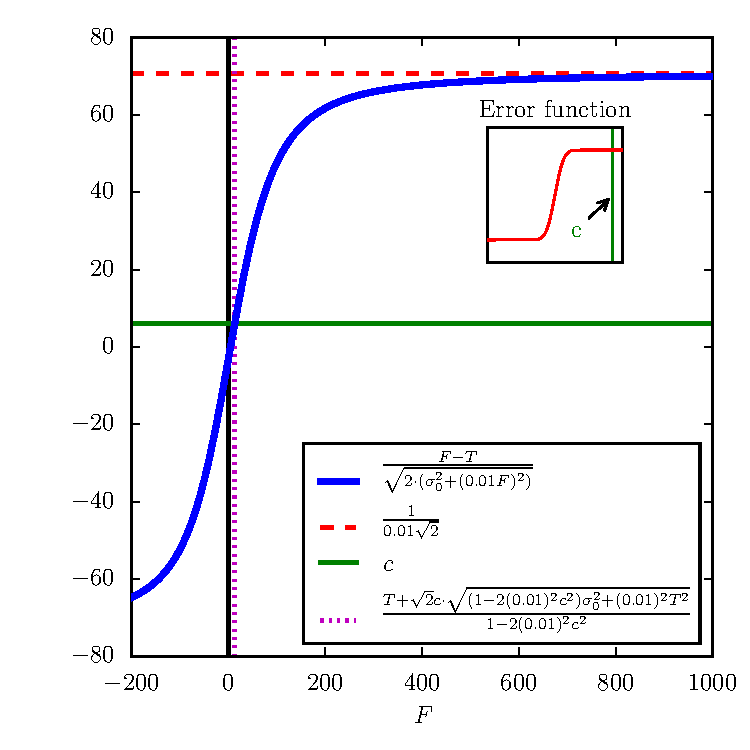
\includegraphics{{fig/erfArg}}
\end{center}
\caption{The argument of the error function in Eq.~\ref{eq:mu_zeta} (blue curve). See text for discussion.}
\label{fig:erfArg}
\end{figure}
